
\chapter{Felhasznált technológiák}

\begin{osszefoglal}
	Ebben a fejezetben, a projekt elkészítése során felhasznált technológiákat ismertetem.
	
\end{osszefoglal}

\section{Android}

\begin{figure}
	\centering
	\setlength{\abovecaptionskip}{0pt}
	\setlength{\belowcaptionskip}{0pt}
	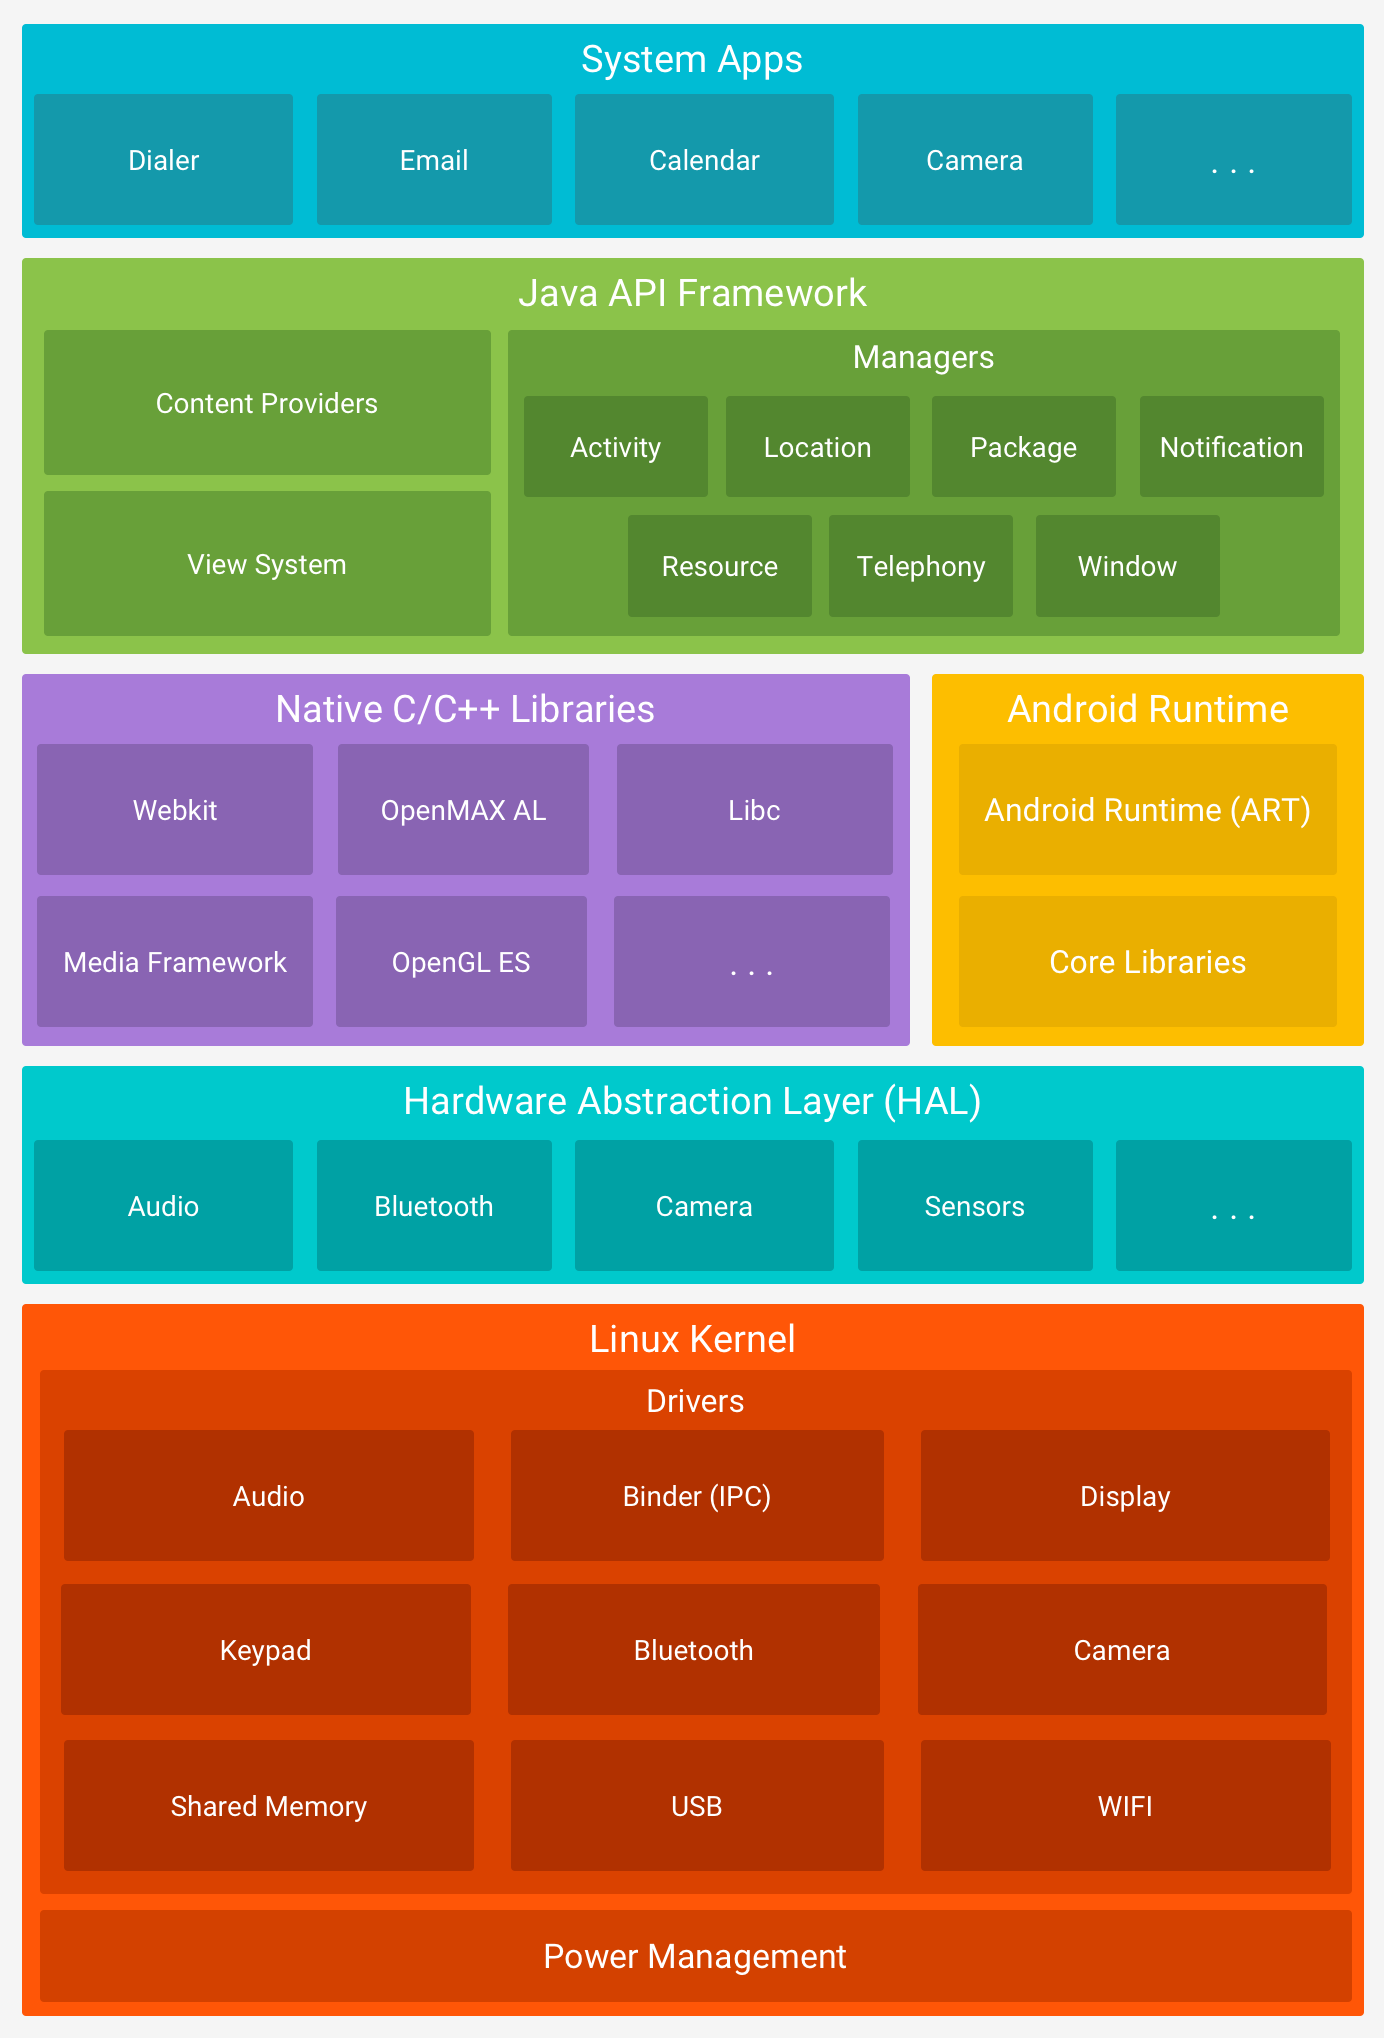
\includegraphics[width=0.9\textwidth, scale=0.9]{images/android}
	 \caption[]%
	{Az Android platform komponensei\\
		{\white .}\hfill\url{https://developer.android.com/guide/platform/}}
\end{figure}

Az Android\cite{android} egy nyílt forráskódú, Linux kernel alapú többfelhasználós operációs rendszer, ahol minden applikáció egy külön felhasználó. Hivatalos nyelvei a Java és a Kotlin. Alapértelmezetten, a rendszer minden applikációnak kioszt egy egyedi Linux felhasználói ID-t (az ID-t csak a rendszer használja, és ismeretlen az applikáció számára). Az operációs rendszer úgy osztja ki a hozzáfárési jogokat az applikáció állományai számára, hogy csak az a felhasználói ID férjen hozzájuk, amivel az adott applikáció rendelkezik. Minden folyamat (process) rendelkezik a saját virtuális gépével, tehát minden applikáció kódja egymástól teljesen izoláltan fut. Alapértelmezetten minden applikáció a saját Linux folyamatában fut. Az Android operációs rendszer elindítja a folyamatot, amikor az applikáció valamelyik komponensének szüksége van rá, majd leállítja azt, mikor többé már nincs rá szükség, vagy ha a rendszernek mermóriát kell lefoglalnia, más applikációk számára. Az Android operációs rendszer “a legkevesebb kiváltság elvét” (“the principle of least privilige”) alkalmazza, tehát alapértelmezetten, minden applikációnak csak azokhoz a komponensekhez van hozzáférése, amik szükségesek a feladatának elvégzéséhez, és semmi egyébhez.

Egy android applikációnak négy fajta komponense lehet: Activity, Service, Broadcast receiver, Content provider. Ezek közül az Activity szolgál a felhasználóval történő interakció eszközéül, ez ugyanis egy felhasználói felülettel rendelkező képernyő. Activity-k, Service-k és Broadcast receiver-ek egy aszinkron üzenet által aktiválódnak, amit Intent-nek (szándék) nevezünk.

Az AndroidManifest.xml egy konfigurációs állomány, ami a projekt gyökér könyvtárában található. Itt vannak deklarálva az applikáció komponensei, valamint a szükséges hozzáférési jogokat is itt kell feltünteni.

\subsection{A Linux kernel}

Az Android platform alapja a Linux kernel (mag). Például az Android Runtime (futási környezet) a Linux magjára támaszkodik olyan funkcionalitásokért, mint a futási szálak kezelése és az alacsony szintű memóriakezelés.

\subsection{Hardware Abstraction Layer (HAL)}

A hardver absztrakciós réteg olyan szabványos interfészeket (interface) biztosít, amelyek segítségével az eszköz hardvereinek funkcionalitásait a Java API keretrendszeren belül használhatjuk. A HAL több könyvtárból, modulból áll, melyek mindegyike implementál egy interfészt valamely hardver-komponens számára, mint például a kamera vagy a bluetooth. Amikor a keretrendszer API egy függvényhívással használatba akarja venni az eszköz hardver-komponensét, akkor az Android operációs rendszer betölti az adott komponenshez tartozó könyvtár modult.

\subsection{Android Runtime}

Azokon az eszközökön, amelyeken az Android 5.0 (API szint 21) vagy újabb verziója fut, minden applikáció a saját folyamatában (process) fut, a saját ART instanciájában. Az ART úgy lett megírva, hogy több virtuális gépet hozzon létre kevés memóriával rendelkező eszközökön úgy, hogy úgynevezet DEX (Dalvik Executable Format) állományokat hajt végre. A DEX egy bájtkód formátum, különösképpen az Android-ra tervezték és arra van optimalizálva, hogy kevés memóriát vegyen igénybe. A build rendszerek a forráskódot DEX bájtkódra fordítják, melyek majd az Android platformon fognak futni.

Az ART főbb funkciói közé tartozik: a futásidejű (JIT), valamint futási idő előtti ( AOT) fordítás, az optimalizált szemétgyűjtés (Garbage Collection). Android 9 (API 28) vagy annál magasabb verziókon az alkalmazás DEX állományai sokkal kompaktabb gépi kóddá vannak átalakítva.

\subsection{Natív C/C++ könyvtárak}

Az Android több alap rendszerkomponense, mint például az ART és a HAL, natív kódban íródtak, melyeknek szükségük van C/C++ könyvtárakra. A Java keretrendszer API segítségével ezeknek a natív könyvtáraknak több funkcionalitását is igénybe vehetjük. Például az OpenGl ES-hez az Android keretrendszer Java OpenGL API-ja segítségével férhetünk hozzá, hogy támogatást nyerjünk a rajzoláshoz, valamint a 2D és 3D grafikák manipulálásához.

\subsection{Java API keretrendszer}

Az Android operációs rendszer funkciói a Java nyelven íródott API-kon keresztül érhetők el. Ezek az API-k az építőelemek, melyek segítségével létrehozhatunk egy applikációt.

\begin{description}
	\setlength{\itemsep}{0.04mm}
	\item[View rendszer] -- felhasználói felületért felelő XML állományok, amik a különböző UI elemeket (gombok, szövegdobozok, konténerek) tartalmazzák.
	\item[Erőforráskezelő (Resource Manager)] -- ez szolgáltatja az alkalmazás által, a forráskódon kívül igénybe vett erőforrásokat, mint például a fordítható karakterláncok, grafikai elemek, alaprajz (layout) fájlok.
	\item[Értesítéskezelő (Notification Manager)] -- engedélyezi az alkalmazások számára, hogy értesítéseket jelenítsenek meg az állapotsorban (status bar).
	\item[Activity-kezelő] -- az applikációk életciklusáért felel, valamint a múltbeli navigációkat is elmenti. Az Activity osztályok a View-k mögötti logikát tartalmazzák.
	\item[Tartalom szolgáltató (Content Provider)] -- segítségével tudnak az alkalmazások egymás adataihoz hozzáférni, vagy megosztani saját adataikat.
\end{description}

\subsection{Rendszer alkalmazások}

Van néhány alkalmazás, ami alapból benne van az Android-ban, ezek többek között az üzenetküldésért, naptárért, internetes böngészésért és a névjegyekért felelnek. A rendszer alkalmazásoknak nincs különleges státuszuk, bármely harmadik féltől származó applikáció átveheti alapértelmezettként az adott funkciók kezeléséért felelő szerepet. Kivételt képez a Beállítások (Settings) alkalmazás. A beépített alkalmazások funkcionalitásait a fejlesztők a saját applikációikban is igénybe vehetik, példa erre a "megosztás SMS-ként", amikor a megosztani kívánt szöveget egy rendszeralkalmazás segítségével küldik el.


\section{Gradle}

A Gradle\cite{gradle} egy nyílt forráskódú projektépítő eszköz (build automation tool). A Groovy, vagy Kotlin nyelvű scriptekbe megadhatjuk a projektünk külső függöségeit (például API-k, library-k), melyeket letölt, majd lekompillálja és lefordítja a forráskódot.

\subsection{Teljesítmény}

\begin{description}
	\setlength{\itemsep}{0.04mm}
	\item[Inkrementális build] -- a Gradle leellenőrzi a build-ek futtatása között, hogy változtak-e a bemeneti adatok, a kimeneti adatok, vagy egy feladat implementációja az utolsó build meghívása óta. Ha nem változtak, akkor a feladatot (task) nem hajtja végre még egyszer. Egy faladat konfigurációja is bemeneti adatként tekintendő.
	\item[Inkrementális részfeladatok] -- részfeladatok esetén is számon tartja, hogy változtak-e a bemeneti, valamint a kimeneti adatok, így pontosan meg tudja állapítani, hogy mi változott, így nem biztos, hogy mindent újra kell build-elnie.
	\item[Párhuzamos végrehajtás] -- lehetőség van a feladatok és a részfeladatok párhuzamos végrehajtására, ami jelentősen növeli a build végrehajtásának sebességét.
	\item[Függőségek párhuzamos letöltése] -- a függőségek letőltése párhuzamosan zajlik, igény szerint, vagyis csak akkor, amikor szükség van ezekre.
\end{description}

\subsection{Függőségkezelés}

\begin{description}
	\setlength{\itemsep}{0.04mm}
	\item[Tranzitív függőségek] -- függőség menedzselő rendszer lévén, a Gradle gondoskodik a tranzitív függőségek letöltéséről, valamint kezeléséről.
	\item[Külső függőségek] -- amikor a függőségek "távoli raktárakban" (remote repository) találhatóak, akkor ezeket eltárolja egy lokálisan, így egymást követő build-ek során újra felhasználja, elkerülvén a felesleges hálózati forgalmat.
\end{description}

\subsection{Android alkalmazások}

Az Andoid Studio-hoz (az android hivatalos fejlesztői környezete) tartozó Gradle kiegészítő az android alkalmazások hivatalos build eszköze, melyet az android fejlesztői csapata tart karban.

\begin{description}
	\setlength{\itemsep}{0.04mm}
	\item[Teljes integráció az Android Studio-val] -- a Gradle olyannyira mélyen van integrálva az Android Studio-ba, hogy az utóbbinak nincs is saját build eszköze, hanem őt bízza meg a build-elési feladatokkal.
	\item[Automatikus aláírás] -- automatikusan aláírja a fejlesztett applikációkat, ami szükséges ahhoz, hogy feltöltsük ezeket a Google Play áruházba.
	\item[Multidex támogatás] -- ez lehetővé teszi, hogy meghaladjuk a 65000-es metódusszám limitet, mely az Anroid DEX állományokra vonatkozik és az applikáció .apk-ba való csomagolásakor történik az ellenőrzése.
\end{description}

\section{Firebase}

\subsection{Autentikáció}

A Firebase Authentication\cite{auth} egy backend (szerver oldali) szolgáltatást nyújt melynek segítségével a felhasználók autentikációját oldhatjuk meg. Az autentikáció módjaként támogatja a jelszó, telefonszám, valamint népszerű indentitás szolgáltatók, mint például a Google, Facebook vagy Twitter használatát. Az aktuális ipari standardokat használja, mint az OAuth 2.0 és az OpenID Connect. Feladatai közé tartozik a regisztráció, bejelentkezés, e-mail cím aktiválása és az elfelejtett jelszó visszaállítása.

\begin{description}
	\setlength{\itemsep}{0.04mm}
	\item[Felhasználók tulajdonságai] -- a Firebase felhasználónak a programozási megfelelője a FirebaseUser osztály. Egy ilyen felhszanáló előre meghatározott attribútumokkal rendelkezik, minden egyéb információt az adatbázisban lehet tárolni. Ezek az alaptulajdonságok az egyedi ID, a fő e-mail cím, a név és egy kép URL. Ha egy felhasználó az e-mail cím/ jelszó kombinációval regisztrál, akkor csak a fő e-mail cím attribútum kap értéket, valamint az egyedi ID is kigenerálódik.
	\item[Aktuális felhasználó] -- amikor egy felhasználó regisztrál vagy bejelentkezik, ő válik az Auth instancia aktuális felhasználójává. A FirebaseAuth tárolja a felhasználó státuszát, így az applikáció újraindításakor nem vesztődik el a felhasználó információja. Ha kijelentkezik, akkor az Auth instancia már nem fogja tovább tárolni FirebaseUser referenciáját, az aktuális felhasználó megszűnik létezni.
	\item[Felhasználói életciklus] -- az Auth listener (figyelő) értesítést kap ha egy felhasználó bejelentkezik, kijelentkezik, a belépési tokenje frissítődik vagy ha az Auth objektum befejezi az inicializálást.
	\item[Autentikációs tokenek] -- A Firebase ID token akkor jön létre, amikor egy felhasználó bejelentkezik egy Firebase applikációba. Ez egy aláírt JSON Web Token (JWT), amely biztonságosan tudja azonosítani a felhasználót egy Firebase projektben. Ezek a tokenek tartalmazzák a felhasználó alapvető információit, mint például az egyedi ID. Ennek segítségével leellenőrizhetjük, hogy ki az éppen bejelentkezett felhasználó.
\end{description}

\subsection{Cloud Firestore}

A felhasználók adatainak, beállításainak tárolására, kezelésére a Cloud Firestore\cite{firestore} nevű no-sql adatbázist használtam, mely a CRUD%
\footnote{ %
	create, read, update, delete
}  %
műveletekhez is biztosít metódusokat. Az adatbázisban található adatokhoz való hozzáférést egy szabállyal kell megadni, amelyet a szerver leellenőriz a CRUD műveletek végrehajtása esetén. Fő adottságai:

\begin{description}
	\setlength{\itemsep}{0.04mm}
	\item[Flexibilitás] -- a Cloud Firestore adatmodellje támogatja a flexibilis, hierarchikus adatsruktúrákat. Az adatokat dokumentumokban tárolja, melyeket kollekciókba lehet rendezni. A dokumentumok komplex, egymásba ágyazott objektumokat is tárolhatnak az alkollekciók mellett. Az adatok kulcs-érték párok, az értékek lehetnek számok, karakterláncok, tömbök, geopontok vagy akár sajátos osztályok. Amennyiben sajátos osztály akarunk használni, annak rendelkeznie kell egy publikus konstruktorral, melynek nincsenek paraméterei, valamint az attribútumokhoz kell tartozzon egy-egy publikus „getter”%
	\footnote{ %
		egy paraméter nélküli metódus, mely egy attribútumot térít vissza - példa: String getName()
	}  %
	metódus.
	\item[Kifejező lekérdezés] -- olyan lekérdezéseket alkalmazhatunk, melyek visszatérítenek egy specifikus dokumentumot, vagy akár az összes dokumentumot a kollekcióból, ami illeszkedik a lekérdezési paraméterekhez. Több szűrőt is alkalmazhatunk, ezek lehetnek láncoltak is, valamint kombináltak a rendezéssel. Az indexelésből kifolyólag a teljesítmény nem az adathalmaztól, hanem az eredményhalmaz méretétől fog függeni.
	\item[Valós idejű frissítések] -- adatszinkronizálást alkalmaz, így az összeköttetésben levő eszközökön mind frissülni fognak az információk.
	\item[Offline támogatás] -- az alkalmazás által használt adatokat cache-eli, így internet nélkül is tudjuk ezeket írni, olvasni. Majd amikor az összeköttetés újra létrejön, a lokális változtatások szinkronizálva lesznek a felhővel.
	\item[Skálázhatóság] -- a Cloud Firestore igénybe veszi a Google Cloud Platform infrastruktúráját. Ezáltal képes automatikus multi-régiós adatreplikációt, erős konzisztencia-garanciát, atomikus batch-műveleteket, valamint valódi tranzakciós támogatottságot nyújtani. 
\end{description}


\section{Térkép}

\subsection{Distance Matrix API}

A Distance Matrix API\cite{distance} egy olyan szolgáltatás, ami visszatéríti az utazási távolságot és időt egy kiindulási és érkezési helyekből álló mátrixhoz. A lekérdezés paraméterei:

\begin{description}
	\setlength{\itemsep}{0.04mm}
	\item[origins (kiindulási pontok)] -- megadhatunk egy földrajzi pontokból álló tömböt, amelyek rendelkeznek szélességi és hosszúsági fok attribútumokkal. Amennyiben karakterláncként adunk meg valódi címeket, a szolgáltatás megpróbálja ezt geokódolni, ezáltal átalakítani az előbb említett formátumba.
	\item[destinations (érkezési pontok)] --  a kiindulási pontokhoz hasonló opciók érvényesek.
	\item[key (kulcs)] -- az applikációhoz tartozó Google fejlesztési kulcs. Ennek segítségével használhatjuk a Google által közzétett API-kat. Mivel egy adott lekérdezés mennyiség után nem ingyenes a szolgáltatás, ezért a web-es felületen lekorlátozhatjuk a fejlesztői kulcsunkhoz való hozzáférést, hogy illetéktelen kezekbe kerülve se szívja le a mérlegünket. A korlátozásokat beállíthjatjuk IP-címre, Android, valamint iOS alkalmazásokra.
	\item[utazási mód (opcionális)] -- vezetés (alapértelmezett), séta, biciklizés, tömegközlekedés.
	\item[mértékegység (opcionális)] -- metrikus (alapértelmezett), birodalmi
\end{description}

Opcionális paraméterként az indulási, érkezési időpontokat szintén megadhatjuk. A lekérdezésre egy JSON (JavaScript Object Notation) vagy egy XML formátumú válasz érkezik, egy jól meghatározott struktúrával:

\begin{description}
	\setlength{\itemsep}{0.04mm}
	\item[státusz] -- amennyiben sikeres volt a lekérdezésunk, válaszul itt OK-t kapunk. Hiba esetén a következő üzenetekkel találkozhatunk: INVALID\_REQUEST (helytelen formátumú kérés), MAX\_ELEMENTS\_EXCEEDED (a kérésenkénti maximális csomópontszám meghaladása), OVER\_DAILY\_LIMIT (hiányzó API kulcs, általunk beállított korlát, érvénytelen fizetési mód), OVER\_QUERY\_LIMIT (a megengedett időintervallumon belül túl sok lekérdezés), REQUEST\_DENIED (a szolgáltatás nem engedélyezi az alkalmazás számára a Distance Matrix használatát), UNKNOWN\_ERROR (szerver oldali hiba).
	\item[kiindulási pontok címei] -- az eredeti lekérdezésből visszatérített objektumok.
	\item[érkezési pontok címei] -- az eredeti lekérdezésből visszatérített objektumok.
	\item[sorok] -- ez tartalmazza az adatokat. Egy adott struktúrájú elemekből álló tömbből áll, ahol az elemek tartalmazzák a státuszt, az időtartamot és a távolságot.
\end{description}

\subsection{Directions API}

A Directions API\cite{directions} meghatározza két helyszín között az leghatékonyabb útvonalat. Alapvetően utazási időre van optimalizálva. A lekérdezés módja a Distance Matrix API-hoz hasonló. A lekérdezésre egy elég bonyolult JSON vagy XML formátumú választ kapunk. Ez magába foglalja a pontokat, melyek segítségével a térképen kirajzolhatjuk az útvonalat, és a navigációhoz szükséges adatokat, információkat.

A PolyUtil osztály segítségével dekódolhatjuk a válaszként érkezett pontokat, majd a Polyline osztály segítségével egy összefüggő vonalként kirajzolhatjuk a térképre.




